\documentclass[12pt, a4paper]{report}
\usepackage{epsfig}
\usepackage{subfigure}
%\usepackage{amscd}
\usepackage{amssymb}
\usepackage{amsbsy}
\usepackage{amsmath}
\usepackage{amsthm}
\usepackage{framed}
\usepackage{subfiles}
%\usepackage[dvips]{graphicx}
\usepackage{natbib}
\bibliographystyle{chicago}
\usepackage{vmargin}
% left top textwidth textheight headheight
% headsep footheight footskip
\setmargins{3.0cm}{2.5cm}{15.5 cm}{22cm}{0.5cm}{0cm}{1cm}{1cm}
\renewcommand{\baselinestretch}{1.5}
\pagenumbering{arabic}
\theoremstyle{plain}
\newtheorem{theorem}{Theorem}[section]
\newtheorem{corollary}[theorem]{Corollary}
\newtheorem{ill}[theorem]{Example}
\newtheorem{lemma}[theorem]{Lemma}
\newtheorem{proposition}[theorem]{Proposition}
\newtheorem{conjecture}[theorem]{Conjecture}
\newtheorem{axiom}{Axiom}
\theoremstyle{definition}
\newtheorem{definition}{Definition}[section]
\newtheorem{notation}{Notation}
\theoremstyle{remark}
\newtheorem{remark}{Remark}[section]
\newtheorem{example}{Example}[section]
\renewcommand{\thenotation}{}
\renewcommand{\thetable}{\thesection.\arabic{table}}
\renewcommand{\thefigure}{\thesection.\arabic{figure}}
\title{Research notes: linear mixed effects models}
\author{ } \date{ }


\begin{document}
	\author{Kevin O'Brien}
	\title{Spring 2011}
	
	\addcontentsline{toc}{section}{Bibliography}
	
	\tableofcontents



%\section{Bartko's Bradley-Blackwood Test}
%
%\begin{itemize}
%	\item The Bradley Blackwood test is a simultaneous test for bias and
%	precision. They propose a regression approach which fits D on M,
%	where D is the difference and average of a pair of results.
%	\item Both beta values, the intercept and slope, are derived from the respective means and
%	standard deviations of their respective data sets.
%	\item We determine if the respective means and variances are equal if
%	both beta values are simultaneously equal to zero. The Test is
%	conducted using an F test, calculated from the results of a
%	regression of D on M.
%	\item We have identified this approach  to be examined to see if it can
%	be used as a foundation for a test perform a test on means and
%	variances individually.
%	\item Russell et al have suggested this method be used in conjunction
%	with a paired t-test , with estimates of slope and intercept.
%\end{itemize}
%subsection{t-test}



\chapter{Formal Models and Tests}



\section{Formal Testing}
The Bland-Altman plot is a simple tool for inspection of the data,
but in itself offers little in the way of formal testing. It is upon the practitioner opinion to judge the outcome of the methodology.

The approach proposed by \citet{BA83} is a formal test on the
Pearson correlation coefficient of case-wise differences and means
($\rho_{AD}$). According to the authors, this test is equivalent
to the `Pitman Morgan Test'. 

For the Grubbs data, the correlation coefficient estimate
($r_{AD}$) is 0.2625, with a 95\% confidence interval of (-0.366,
0.726) estimated by Fishers `r to z' transformation \citep{Cohen}.
The null hypothesis ($\rho_{AD}$ =0) would fail to be rejected.
Consequently the null hypothesis of equal variances of each method
would also fail to be rejected.
There has
no been no further mention of this particular test in
\citet{BA86}, although \citet{BA99} refers to Spearman's rank
correlation coefficient. \citet{BA99} comments `we do not see a
place for methods of analysis based on hypothesis testing'.
\citet{BA99} also states that consider structural equation models
to be inappropriate.


	\section{Classical model for single measurements}
	
	
	Before continuing, we require a simple model to describe a measurement by method $m$. \citet{BXC2004} presents a model to describe the relationship between a value of measurement and its
	real value. The non-replicate case is considered first, as it is the context of the Bland Altman plots. This model assumes that inter-method bias is the only difference between the two methods.
	
	This model is based on measurements $y_{mi}$ by method $m=1,2$ on item $i = 1,2 \ldots$. We use the term $item$ to denote an individual, subject or sample, to be measured, being randomly sampled from a population
	% Let $y_{mi}$ be the $y_{mi}$ by method $m=1,2$ on item $i = 1,2 \ldots$
	\begin{equation}
	y_{mi}  = \alpha_{m} + \mu_{i} + e_{mi}, \qquad  e_{mi} \sim
	\mathcal{N}(0,\sigma^{2}_{m}).
	\end{equation}
	
	Here $\alpha_m$ is the fixed effect associated with method $m$,
	$\mu_i$ is the true value for subject $i$ (fixed effect) and $e_{mi}$ is a random effect term for errors.
	
%	The case-wise differences are expressed as $d_{i} = y_{1i} - y_{2i}$. Even though the separate variances can not be identified, their sum can be estimated by the empirical variance of the differences, using standard statistical theory. The covariance matrix for case-wise differences can be specified as
%	\[
%	\Sigma = \left( \begin{array}{cc}
%	\sigma^2_1 + \sigma^2_2 &  \frac{1}{2}(\sigma^2_1 - \sigma^2_2) \\
%	\frac{1}{2}(\sigma^2_1 - \sigma^2_2) &   \sigma^2_b + \frac{1}{4}(\sigma^2_1 + \sigma^2_2)
%	\end{array}\right).
%	\]
	The case-wise differences and means are calculated as $d_{i} =
	x_{i}-y_{i}$ and $a_{i} = (x_{i}+y_{i})/2$  respectively. Both
	$d_{i}$ and $a_{i}$ are assumed to follow a bivariate normal
	distribution with $E(d_{i})= \mu_{d} = \mu_{1} - \mu_{2}$ and
	$E(a_{i})= \mu_{a} = (\mu_{1} + \mu_{2})/2$. The variance matrix
	$\Sigma_{(a,d)}$ is
	
	\begin{eqnarray}
	\Sigma_{(a,d)}= \left[\begin{matrix}
	\sigma^{2}_{1}+\sigma^{2}_{2}&\frac{1}{2}(\sigma^{2}_{1}-\sigma^{2}_{2})\\
	\frac{1}{2}(\sigma^{2}_{1}-\sigma^{2}_{2})&\sigma^{2}+
	\frac{1}{4}(\sigma^{2}_{1}+\sigma^{2}_{2})
	\end{matrix} \right].
	\end{eqnarray}
		
	Likewise the separate $\alpha$ can not be estimated, only their difference can be estimated as $\bar{d}$ (i.e. the inter-method bias). This model implies that the difference between the paired measurements can be expressed as
	\[ d_{i} = y_{1i} - y_{2i} \sim \mathcal{N} (\alpha_{1} - \alpha_{2}, \sigma^2_{1} + \sigma^2_{2}). \]
	Importantly, this is independent of the item levels $\mu_i$. As the case-wise differences are of interest, the parameters of interest are the fixed effects for methods $\alpha_{m}$.
	
	% \[ y_{mi} =  \alpha_{m}  + \mu_{i} + e_{mi}  \]
	% Importantly these variance covariance structures are central to ARoy2009 methodology.
	% \citet{ARoy2009} proposes a series of hypothesis tests based on these matrices as part of her methodology. These tests shall be reverted to in due course.
	
	%	The standard deviation of the differences of variables $a$ and $b$ is computed as
	%	\[
	%	\mbox{var}(a - b) = \mbox{var} ( a )  + \mbox{var} ( b ) - 2\mbox{cov} ( a ,b )
	%	\]
	
	

\section{Model for single measurement observations}
\citet{Kinsella} formulates a model for
single measurement observations for a method comparison study as a
linear mixed effects model, i.e. model that additively combine
fixed effects and random effects.
\[
Y_{ij} =\quad \mu + \beta_{j} + u_{i} + \epsilon_{ij} \qquad i = 1,\dots,n
\qquad j=1,2\]

The true value of the measurement is represented by $\mu$ while the fixed effect due to method $j$ is $\beta_{j}$.
For simplicity these terms can be combined into single terms; $\mu_{1} = \mu+ \beta_{1}$ and $\mu_{2} = \mu + \beta_{2}$. The inter-method bias is the difference of the two fixed effect terms, $\beta_{1}-\beta_{2}$. Each individual is assumed to give rise to a random error, represented by $u_{i}$. This random effects term is assumed to have mean zero and be normally distributed with variance $\sigma^2$. There is assumed to be an attendant error for each measurement on each individual, denoted $\epsilon_{ij}$. This is also assumed to have mean zero. The variance of measurement error for both methods are not assumed to be identical for both methods variance,  hence it is denoted $\sigma^2_{j}$. The set of observations ($x_{i},y_{i}$) by methods $X$ and $Y$ are assumed to follow a bivariate normal distribution with expected values $E(x_{i})= \mu_{i}$ and $E(y_{i})= \tau_{i}$ respectively. The variance covariance of the observations $\boldsymbol{\Sigma}$ is given by

\[
\boldsymbol{\Sigma} = \left[
\begin{array}{cc}
\sigma^{2} + \sigma^{2}_{1} & \sigma^{2} \\
\sigma^{2} & \sigma^{2} + \sigma^{2}_{2} \\
\end{array}
\right]
\] 
% The inter-method bias is the difference of the two fixed effect terms, $\beta_{1}-\beta_{2}$.



%%%%%%%%%%%%%%%%%%%%%%%%%%%%%%%%%%%%%%%%%%%%%%%%%%%%%%%%%%%%%%%%%%%%%%%%%%%%%%%%%%%%%%


\section{Morgan Pitman}


An early contribution to formal testing in method comparison was
made by both \citet{Morgan} and \citet{Pitman}, in separate
contributions. This test assess the equality
of population variances. Pitman's test tests for zero correlation
between the sums and products. The basis of this approach is that the
distribution of the original measurements is bivariate normal.
Correlation between differences and means is a test statistics for
the null hypothesis of equal variances given bivariate normality.


The test of the hypothesis that the variances $\sigma^2_1$ and $\sigma^2_2$ are equal, which was devised concurrently by \citet{Pitman} and \citet{Morgan}, 
is based on the correlation of the casewise-differences and sums, $d$ with $s,$ the coefficient being $ \rho_{(d,s)} = (\sigma^2_1 -\sigma^2_2) / ( \sigma_D \sigma_S ),$ which is zero if, and only
if, $\sigma^2_1 = \sigma^2_2.$ The classical Pitman-Morgan test can be adapted for the correlation value $\rho_{(a,d)}$ ,and
is evaluated as follows;

\begin{equation}
\rho(a,d)=\quad\frac{\sigma^{2}_{1}-\sigma^{2}_{2}}{\sqrt{(\sigma^{2}_{1}+\sigma^{2}_{2})(4\sigma^{2}_{S}+\sigma^{2}_{1}+\sigma^{2}_{2})}}
\end{equation}
The basis of this approach is that the
distribution of the original measurements is bivariate normal.
Morgan and Pitman noted that the correlation coefficient depends
upon the difference $\sigma^{2}_{1}- \sigma^{2}_{2}$, being zero
if and only if $\sigma^{2}_{1}=\sigma^{2}_{2}$.

The test of the hypothesis that the variance of both methods are
equal is based on the correlation value $\rho_{D,A}$ which is
evaluated as follows;

\begin{equation}
\rho(D,A)=\quad\frac{\sigma^{2}_{1}-\sigma^{2}_{2}}{\sqrt{(\sigma^{2}_{1}+\sigma^{2}_{2})(4\sigma^{2}_{S}+\sigma^{2}_{1}+\sigma^{2}_{2})}}
\end{equation}

The correlation constant takes the value zero if, and only if, the
two variances are equal. Therefore a test of the hypothesis $H:
\sigma^{2}_{1}=\sigma^{2}_{2}$ is equivalent to a test of the
hypothesis $H: \rho(D,A) = 0$. The corresponds to the well-known
$t$ test for a correlation coefficient with $n-2$ degrees of
freedom.

The classical Pitman-Morgan test is a hypothesis test for equality of the variance of two data sets; $\sigma^{2}_{1} =
\sigma^{2}_{2}$, based on the correlation value $\rho_{a,d}$ ,and is evaluated as follows;

\begin{equation}
\rho(a,d)=\quad\frac{\sigma^{2}_{1}-\sigma^{2}_{2}}{\sqrt{(\sigma^{2}_{1}+\sigma^{2}_{2})(4\sigma^{2}_{S}+\sigma^{2}_{1}+\sigma^{2}_{2})}}
\end{equation}

The correlation constant takes the value zero if, and only if, the
two variances are equal. 

Morgan and Pitman noted that the correlation coefficient depends
upon the difference $\sigma^{2}_{1}- \sigma^{2}_{2}$, being zero
if and only if $\sigma^{2}_{1}=\sigma^{2}_{2}$.
Therefore a test of the hypothesis $H: \sigma^{2}_{1}=\sigma^{2}_{2}$ is equivalent to a test of the hypothesis $H: \rho(D,A) = 0$. This corresponds to the well-known $t$ test for a correlation coefficient with $n-2$ degrees of freedom. 


\citet{Bartko} describes the Morgan-Pitman test as identical to the test of the slope equal to zero in the regression of $Y_{i1}$ on $Y_{12}$, a result that can be derived using straightforward algebra. The Pitman-Morgan test is equivalent to the marginal test of the slope estimate in Bradley-Blackwood’s model.






The Pitman-Morgan test for equal variances is based on the correlation of D with S. The correlation coefficient is zero if, and only if, the variances are equal. The test statistic is the familiar t-test with n-2 degree of freedom.

Bradley and Blackwood (1989) construct the conditional expectation of D given S as linear model.  They used this result to propose a test of the joint hypothesis of the mean difference and equal variances. 
If the intercept and slope estimates are zero, the two methods have the same mean and variance.






\section{Identifiability}
\citet{DunnSEME} highlights an important issue regarding using models such as structural equation modelling, which is the identifiability problem. This comes as a
result of there being too many parameters to be estimated. Therefore assumptions about some parameters, or estimators used, must be made so that others can be estimated. For example, in the literature, the variance ratio $\lambda=\frac{\sigma^{2}_{1}}{\sigma^{2}_{2}}$
must often be assumed to be equal to $1$ \citep{linnet98}. \citet{DunnSEME} considers approaches based on two methods with single measurements on each subject as inadequate for a serious
study on the measurement characteristics of the methods. This is because there would not be enough data to allow for a meaningful
analysis. There is, however, a counter-argument that in many practical settings it is very difficult to get replicate observations when, for example, the measurement method requires invasive medical
procedure.

%%%%%%%%%%%%%%%%%%%%%%%%%%%%%%%%%%%%%%%%%%%%%%%%%%%%%%%%%%%%%%%%%%%%%%%%%%%%%%%



%This application of the
%Grubbs method presumes the existence of this condition, and necessitates
%replication of observations by means external to and independent of the first
%means. The Grubbs estimators method is based on the laws of propagation of
%error. By making three independent simultaneous measurements on the same
%physical material, it is possible by appropriate mathematical manipulation of
%the sums and differences of the associated variances to obtain a valid
%estimate of the precision of the primary means. Application of the Grubbs
%estimators procedure to estimation of the precision of an apparatus uses
%the results of a physical test conducted in such a way as to obtain a series
%of sets of three independent observations.





\section{Measurement Error Models}
\citet{DunnSEME} proposes a measurement error model for use in
method comparison studies. Consider n pairs of measurements
$X_{i}$ and $Y_{i}$ for $i=1,2,...n$.
\begin{equation}
X_{i} = \tau_{i}+\delta_{i}\\
\end{equation}
\begin{equation}
Y_{i} = \alpha +\beta\tau_{i}+\epsilon_{i} \nonumber
\end{equation}

In the above formulation is in the form of a linear structural
relationship, with $\tau_{i}$ and $\beta\tau_{i}$ as the true
values , and $\delta_{i}$ and $\epsilon_{i}$ as the corresponding
measurement errors. In the case where the units of measurement are
the same, then $\beta =1$.

\begin{equation}
E(X_{i}) = \tau_{i}\\
\end{equation}
\begin{equation}
E(Y_{i}) = \alpha +\beta\tau_{i} \nonumber
\end{equation}
\begin{equation}
E(\delta_{i}) = E(\epsilon_{i}) = 0 \nonumber
\end{equation}

The value $\alpha$ is the inter-method bias between the two
methods.

\begin{eqnarray}
z_0 &=& d = 0 \\
z_{n+1} &=& z_n^2+c
\end{eqnarray}




	\section{Move to Chapter 3}
	\citet{BXC2004} also advocates the use of linear mixed models in
	the study of method comparisons. The model is constructed to
	describe the relationship between a value of measurement and its
	real value. The non-replicate case is considered first, as it is
	the context of the Bland-Altman plots. This model assumes that
	inter-method bias is the only difference between the two methods.
	A measurement $y_{mi}$ by method $m$ on individual $i$ is
	formulated as follows;
	\begin{equation}
	y_{mi}  = \alpha_{m} + \mu_{i} + e_{mi} \qquad ( e_{mi} \sim
	N(0,\sigma^{2}_{m}))
	\end{equation}
	The differences are expressed as $d_{i} = y_{1i} - y_{2i}$ For the
	replicate case, an interaction term $c$ is added to the model,
	with an associated variance component. All the random effects are
	assumed independent, and that all replicate measurements are
	assumed to be exchangeable within each method.
	
	\begin{equation}
	y_{mir}  = \alpha_{m} + \mu_{i} + c_{mi} + e_{mir} \qquad ( e_{mi}
	\sim N(0,\sigma^{2}_{m}), c_{mi} \sim N(0,\tau^{2}_{m}))
	\end{equation}
	

\section{Carstensen Model for Replicate Measurements}


\citet{BXC2008} develop their model from a standard two-way analysis of variance model, reformulated for the case of replicate measurements, with random effects terms specified as appropriate. 
For the replicate case, an interaction term $c$ is added to the model, with an associated variance component. Their model describing $y_{mir} $, again the $r$th replicate measurement on the $i$th item by the $m$th method ($m=1,2,$ $i=1,\ldots,N,$ and $r = 1,\ldots,n$), can be written as
\begin{equation}\label{BXC-model}
y_{mir}  = \alpha_{m} + \mu_{i} + a_{ir} + c_{mi} + \epsilon_{mir}.
\end{equation}
Again, the fixed effects $\alpha_{m}$ and $\mu_{i}$  represent the intercept for method $m$ and the `true value' for item $i$ respectively. The random-effect terms comprise an item-by-replicate interaction term $a_{ir} \sim \mathcal{N}(0,\varsigma^{2})$, a method-by-item interaction term $c_{mi} \sim \mathcal{N}(0,\tau^{2}_{m}),$ and model error terms $\varepsilon \sim \mathcal{N}(0,\varphi^{2}_{m}).$ All random-effect terms are assumed to be independent. For the case when replicate measurements are assumed to be exchangeable for item $i$, $a_{ir}$ can be removed.

The model expressed in (2) describes measurements by $m$ methods, where $m = \{1,2,3\ldots\}$. Based on the model expressed in (2), \citet{BXC2008} compute the limits of agreement as
\[
\alpha_1 - \alpha_2 \pm 2 \sqrt{ \tau^2_1 +  \tau^2_2 +  \varphi^2_1 +  \varphi^2_2 }
\]
\citet{BXC2008} notes that, for $m=2$, separate estimates of $\tau^2_m$ can not be obtained. To overcome this, the assumption of equality, i.e. $\tau^2_1 = \tau^2_2$ is required.
\begin{equation}
y_{mir}  = \alpha_{m} + \mu_{i} + c_{mi} + e_{mir}, \qquad  e_{mi}
\sim \mathcal{N}(0,\sigma^{2}_{m}), \quad c_{mi} \sim \mathcal{N}(0,\tau^{2}_{m}).
\end{equation}

%Of particular importance is terms of the model, a true value for item $i$ ($\mu_{i}$).  The fixed effect of Roy's model comprise of an intercept term and fixed effect terms for both methods, with no reference to the true value of any individual item. 
%A distinction can be made between the two models: Roy's model is a standard LME model, whereas Carstensen's model is a more complex additive model.







\section{Paired sample \emph{t} test}

\citet{Bartko} discusses the use of the well known paired sample
$t$ test to test for inter-method bias; $H: \mu_{d}=0$. The test
statistic is distributed a $t$ random variable with $n-1$ degrees
of freedom and is calculated as follows,

\begin{equation}
t^{*} = \frac{\bar{d}}{ \frac{s_{d}}{\sqrt{n}}}
\end{equation}

where $\bar{d}$ and $s_{d}$ is the average of the differences of
the $n$ observations. Only if the two methods show comparable
precision then the paired sample student $t$-test is appropriate for
assessing the magnitude of the bias.




	\chapter{Regression Procedures}
	
	%================================================================================================= %
	\section{Regression Methods}
	Conventional regression models are estimated using the ordinary
	least squares (OLS) technique, and are referred to as `Model I
	regression' \citep{CornCoch,ludbrook97}. A key feature of Model I
	models is that the independent variable is assumed to be measured
	without error. As often pointed out in several papers
	\citep{BA83,ludbrook97}, this assumption invalidates simple linear
	regression for use in method comparison studies, as both methods
	must be assumed to be measured with error.
	
	The use of regression models that assumes the presence of error in
	both variables $X$ and $Y$ have been proposed for use instead
	\citep{CornCoch,ludbrook97}. These methodologies are collectively
	known as `Model II regression'. They differ in the method used to
	estimate the parameters of the regression.
	
	Regression estimates depend on formulation of the model. A
	formulation with one method considered as the $X$ variable will
	yield different estimates for a formulation where it is the $Y$
	variable. With Model I regression, the models fitted in both cases
	will entirely different and inconsistent. However with Model II
	regression, they will be consistent and complementary.
	
	Regression approaches are useful for a making a detailed examination of the biases across the range of measurements, allowing bias to be decomposed into fixed bias and proportional bias.
	Fixed bias describes the case where one method gives values that are consistently different
	to the other across the whole range. Proportional
	bias describes the difference in measurements getting progressively greater, or smaller, across the range of measurements. A measurement method may have either an attendant fixed bias or proportional bias, or both. \citep{ludbrook}. Determination of these biases shall be discussed in due course.
	
	
	


\subsection{Decomposition of Inter-Method Bias}
Regression approaches are useful for a making a detailed examination of the biases across the range of measurements, allowing inter-method bias to be decomposed into fixed bias and proportional bias. Fixed bias describes the case where one method gives values that are consistently different to the other across the whole range. 

%The Intercept and Slope can provide estimates for the constant bias and proportional bias occurring between both methods.

Constant or proportional bias in method comparison studies using linear regression can be detected by an individual test on the intercept or the slope of the line regressed from the results of the two methods to be compared.


Proportional bias describes the difference in measurements getting progressively greater, or smaller, across the range of measurements. A measurement method may have either an attendant fixed bias or proportional bias, or both \citep{ludbrook02}.

If the basic assumptions underlying linear regression are not met, the regression equation, and consequently the estimations of bias are undermined. Outliers are a source of error in regression estimates.
% Determination of these biases shall be discussed in due course.

\subsection{Inference Procedures}
A $95\%$ confidence interval for the intercept estimate can be used to test the intercept, and hence fixed bias, is equal to
zero. This hypothesis is accepted if the confidence interval for the estimate contains the value $0$ in its range. Should this be,
it can be concluded that fixed bias is not present. Conversely, if the hypothesis is rejected, then it is concluded that the
intercept is non zero, and that fixed bias is present.

Testing for proportional bias is a very similar procedure. The $95\%$ confidence interval for the slope estimate can be used to
test the hypothesis that the slope is equal to $1$. This hypothesis is accepted if the confidence interval for the estimate
contains the value $1$ in its range. If the hypothesis is rejected, then it is concluded that the slope is significant
different from $1$ and that a proportional bias exists.


	\section{Incorrect Techniques: Simple Linear Regression}
	
	
	\subsection{Regression Analysis}
	Another inappropriate approach is the regressing one set of measurements against the other. According to this methodology the measurement methods could considered equivalent if the confidence interval for
	the regression coefficient included $1$. Analysts sometimes use least squares (referred to by Ludbrook as Model I) regression analysis to calibrate one method of measurement against another. In this technique, the sum of the squares of the vertical deviations of y values from the line is minimized. This approach is invalid, because both y and x values are attended by random error.
	
	
	\subsection{The Identity Plot} This is a simple graphical approach, advocated by \citet{BA86}, that yields a cursory examination of how well the measurement methods agree. In the case of good agreement, the co-variates of the plot accord closely with the $X=Y$ line.
	
	
	\subsection{Advantages of Regression Approaches for MCS}
	\begin{itemize}
		\item These methods can be employed in conversion problems.
		\item Bland and Altman have stated that regression analysis offers insights into MCS problems.
	\end{itemize}
	\subsection{Disadvantages}
	\begin{itemize}
		\item Regression methods are uninformative about the variability of the differences.
	\end{itemize}
	
	\begin{itemize}\item
		Regression methods can determine the presence of bias, and the levels of constant bias and proportional bias thereof \cite{ludbrook97,ludbrook02}.
	\end{itemize}
	
	
	\begin{itemize}
		\item \textbf{Constant Bias} This is a form of systematic deviations estimated as the average difference between the test
		and the reference method.
		\item \textbf{Proportional Bias} Two methods may agree on average, but they may exhibit differences over a range of measurements.
	\end{itemize}
	
	Two methods may agree on
	average, but they may exhibit differences over a range of measurements.	Proportional Bias is a difference in the two measures which is proportional to the scale of the measurement. 
	
	Using a naive estimation of bias, such as the mean of differences, it may incorrectly indicate absence of bias, by yielding a mean difference close to zero. This would be caused by positive differences in the measurements at one end of the range of measurements being canceled out by negative differences at the other end of the scale.
	
	%------------------------------------------------------------------------%
	
	
	%%%%%%%%%%%%%%%%%%%%%%%%%%%%%%%%%%%%%%%%%%%%%%%%%%%%%%%%%%%%%%%%%%%%%%%%%%%%%%%%%%%%%%%%%%%%%%%%%%%%%%%%%%%%%%%%%%%%%
	\section{Blackwood-Bradley Model} 
\citet{BB89} offers a formal simultaneous hypothesis test for the
mean and variance of two paired data sets. Using simple linear
regression of the differences of each pair against the sums, a
line is fitted to the model, with estimates for intercept and
slope ($\hat{\beta}_{0}$ and $\hat{\beta}_{1}$). The null
hypothesis of this test is that the mean ($\mu$) and variance
($\sigma^{2}$) of both data sets are equal if the slope and
intercept estimates are equal to zero(i.e $\sigma^{2}_{1} =
\sigma^{2}_{2}$ and $\mu_{1}=\mu_{2}$ if and only if $\beta_{0}=
\beta_{1}=0$ )	

	
	\citet{BB89} have developed a regression based procedure for
	assessing the agreement. This approach performs a simultaneous test for the equivalence of
	means and variances of the respective methods. The Bradley Blackwood test is a simultaneous test for bias and
	precision. They propose a regression approach which fits D on M,
	where D is the difference and average of a pair of results. Using simple linear
	regression of the differences of each pair against the sums, a
	line is fitted to the model, with estimates for intercept and
	slope ($\hat{\beta}_{0}$ and $\hat{\beta}_{1}$).
	%We have identified
	%this approach  to be examined to see if it can be used as a %foundation for a test perform a test on
	%means and variances individually.
	\begin{equation}
	D = (X_{1}-X_{2})
	\end{equation}
	\begin{equation}
	M = (X_{1} + X_{2}) /2
	\end{equation}
	The Bradley Blackwood Procedure fits D on M as follows:\\
	\begin{equation}
	D = \beta_{0} + \beta_{1}M
	\end{equation}
	This technique offers a formal simultaneous hypothesis test for the
	mean and variance of two paired data sets.  The null
	hypothesis of this test is that the mean ($\mu$) and variance
	($\sigma^{2}$) of both data sets are equal if the slope and
	intercept estimates are equal to zero(i.e $\sigma^{2}_{1} =
	\sigma^{2}_{2}$ and $\mu_{1}=\mu_{2}$ if and only if $\beta_{0}=
	\beta_{1}=0$ )
	
	Both beta values, the intercept and slope, are derived from the respective means and
	standard deviations of their respective data sets.
	
	We determine if the respective means and variances are equal if
	both beta values are simultaneously equal to zero. The Test is
	conducted using an F test, calculated from the results of a
	regression of D on M.
	
	
	\textbf{Russell et al} have suggested this method be used in conjunction with a paired t-test , with estimates of slope and intercept.
	
	Bradley and Blackwood have developed a regression based approach
	assessing the agreement.
	
	We have identified this approach  to be examined to see if it can
	be used as a foundation for a test perform a test on means and variances individually.
	
	
	\section{Bradley-Blackwood Method}
	
	
	A test statistic is then calculated from the regression analysis
	of variance values \citep{BB89} and is distributed as `$F$' random
	variable. The degrees of freedom are $\nu_{1}=2$ and $\nu_{1}=n-2$
	(where $n$ is the number of pairs). The critical value is chosen
	for $\alpha\%$ significance with those same degrees of freedom.
	\citet{Bartko} amends this methodology for use in method
	comparison studies, using the averages of the pairs, as opposed to
	the sums, and their differences. This approach can facilitate
	simultaneous usage of test with the Bland-Altman methodology.
	Bartko's test statistic take the form:
	\[ F.test = \frac{(\Sigma d^{2})-SSReg}{2MSReg}
	\]

	
	\subsection{Application to the Grubbs' Data}
	For the Grubbs data, $\Sigma d^{2}=5.09 $, $SSReg = 0.60$ and
	$MSreg=0.06$ Therefore the test statistic is $37.42$, with a
	critical value of $4.10$. Hence the means and variance of the
	Fotobalk and Counter chronometers are assumed to be simultaneously
	equal.
	
	Importantly, this approach determines whether there is both
	inter-method bias and precision present, or alternatively if there
	is neither present. It has previously been demonstrated that there
	is a inter-method bias present, but as this procedure does not
	allow for separate testing, no conclusion can be drawn on the
	comparative precision of both methods.
	
	
	
	% latex table generated in R 2.6.0 by xtable 1.5-5 package
	% Mon Aug 31 15:53:51 2009
	\begin{table}[ht]
		\begin{center}
			\begin{tabular}{lrrrrr}
				\hline
				& Df & Sum Sq & Mean Sq & F value & Pr($>$F) \\
				\hline
				Averages & 1 & 0.04 & 0.04 & 0.74 & 0.4097 \\
				Residuals & 10 & 0.60 & 0.06 &  &  \\
				\hline
			\end{tabular}
			\caption{Regression ANOVA of case-wise differences and averages
				for Grubbs Data}
		\end{center}
	\end{table}
	
	

	\section{Bradley-Blackwood Test (Kevin Hayes Talk)}
	%--------------------------------------------------------------------%
	% KH - UW
	
	This work considers the problem of testing $\mu_1$ = $\mu_2$ and $\sigma^2_1 = \sigma^2_2$ using a random sample from a bivariate normal distribution with parameters $(\mu_1, \mu_2, \sigma^2_1, \sigma^2_2, \rho)$. 
	
	The new contribution is a decomposition of the Bradley-Blackwood test statistic (\textit{Bradley and Blackwood, 1989})for the simultaneous test of {$\mu_1$ = $\mu_2$; $\sigma^2_1 = \sigma^2_2$}  as a sum of two statistics. 
	
	One is equivalent to the Pitman-Morgan (\textit{Pitman, 1939; Morgan, 1939}) test statistic 
	for $\sigma^2_1 = \sigma^2_2$ and the other one is a new alternative to the standard paired-t test of $\mu_D = \mu_1 = \mu_2 = 0$. 
	
	Surprisingly, the classic Student paired-t test makes no assumptions about the equality (or otherwise) of the 
	variance parameters. 
	
	The power functions for these tests are quite easy to derive, and show that when $\sigma^2_1 = \sigma^2_2$, 
	the paired t-test has a slight advantage over the new alternative in terms of power, but when $\sigma^2_1 \neq \sigma^2_2$, the 
	new test has substantially higher power than the paired-t test.
	
	While Bradley and Blackwood provide a test on the joint hypothesis of equal means and equal variances their regression based approach does not separate these two issues.
	
	The rejection of the joint hypothesis may be 
	due to two groups with unequal means and unequal variances; unequal means and equal variances, or equal means and unequal variances. We propose an approach for resolving this (model selection) problem in a manner controlling the magnitudes of the relevant type I error probabilities.
	
	
	

\section{Error-In-Variable Models}
Conventional regression models are estimated using the ordinary
least squares (OLS) technique, and are referred to as `Model I
regression' \citep{CornCoch,ludbrook97}. A key feature of Model I
models is that the independent variable is assumed to be measured
without error. As often pointed out in several papers
\citep{BA83,ludbrook97}, this assumption invalidates simple linear
regression for use in method comparison studies, as both methods
must be assumed to be measured with error.

The use of regression models that assumes the presence of error in
both variables $X$ and $Y$ have been proposed for use instead
\citep{CornCoch,ludbrook97}. These methodologies are collectively
known as ``Error-In-Variables Models" and ``Model II regression". They differ in the method used to
estimate the parameters of the regression.

Errors-in-variables models or measurement errors models are regression models that account for measurement errors in the independent variables, as well as the dependent variable.


Regression estimates depend on formulation of the model. A
formulation with one method considered as the $X$ variable will
yield different estimates for a formulation where it is the $Y$
variable. With Model I regression, the models fitted in both cases
will entirely different and inconsistent. However with Model II
regression, they will be consistent and complementary.

\citet{CornCoch} comparing the three methods, citing studies by other authors, concluding that Deming regression is the most useful of these methods. They found the Bartlett method to be
flawed in determining slopes.

However the author point out that \emph{ clinical laboratory measurements usually increase in absolute imprecision when larger values are measured.} However one of the assumptions that underline Deming and Mandel regression is constancy of the measurement errors throughout the range of values.





	\section{Deming Regression}
	
	As stated previously, the fundamental flaw of simple linear regression is that it allows for measurement error in one variable only. This causes a downward biased slope estimate.
	
	Deming regression is a regression fitting approach that assumes error in both variables. Deming regression is recommended by \citet*{CornCoch} as the
	preferred Model II regression for use in method comparison studies.
	The sum of squared distances from measured sets of values to the regression line is minimized at an angles specified by the ratio $\lambda$ of the residual variance of both variables. I
	When $\lambda$ is one, the angle is 45 degrees. In ordinary linear regression, the distances are minimized in the vertical directions \citep{linnet99}.
	In cases involving only single measurements by each method, $\lambda$ may be unknown and is therefore assumes a value of one. While this will produce biased estimates, they are less biased than ordinary linear regression.
	
	The Bland Altman Plot is uninformative about the comparative influence of proportional bias and fixed bias. Model II approaches, such as Deming regression,  can provide independent tests for
	both types of bias.

As with conventional regression methodologies, Deming regression calculates an estimate for both the slope and intercept for the
fitted line, and standard errors thereof. Therefore there is sufficient information to carry out hypothesis tests on both
estimates, that are informative about presence of fixed and proportional bias.

Deming regression method also calculates a line of best fit for two sets of data. It differs from simple linear regression in that it is derived in a way that factors in for error in the x-axis, as well as the y-axis. The sum of the square of the residuals of both variables are simultaneously minimized. This derivation results in the best fit to minimize the sum of the squares of the perpendicular distances from the data points. Normally distributed error of both variables is assumed, as well as a constant level of imprecision throughout the range of measurements.


\subsection{Kummel's Estimates}


For a given $\lambda$, \citet{Kummel} derived the following estimate that would later be used for the Deming regression slope
parameter. The intercept estimate $\alpha$ is simply estimated in the same way as in conventional linear
regression, by using the identity $\bar{Y}-\hat{\beta}\bar{X}$;
\begin{equation}
\hat{\beta} =\quad \frac{S_{yy} - \lambda S_{xx}+[(S_{yy} -
	\lambda S_{xx})^{2}+ 4\lambda S^{2}_{xy}]^{1/2}}{2S_{xy}}
\end{equation},
with $\lambda$ as the variance ratio. As stated previously $\lambda$ is often unknown, and therefore must be assumed to equal one. 

The sum of squared distances from measured sets of values to the regression line is minimized at an angles specified by the ratio $\lambda$ of the residual variance of both variables. The measurement error is specified with measurement error variance related as 
\[\lambda = \sigma^2_y/\sigma^2_x\]

where $\sigma^2_x$ and $\sigma^2_y$ is the measurement error variance of the $x$ and $y$ variables, respectively.
The variance of the ratio,$\lambda$, specifies the angle.  When $\lambda$ is one, the angle is 45 degrees. 
%In ordinary linear regression, the distances are minimized in the vertical directions \citep{linnet99}. 
This approach would be appropriate when errors in $y$ and $x$ are both caused by measurements, and the accuracy of measuring devices or procedures are known. In cases involving only single measurements by each method, $\lambda$ may be unknown and is therefore assumes a value of one. While this will bias the estimates, it is less biased than ordinary linear regression.

Deming regression assumes that the ratio $\lambda = \sigma^2_{\epsilon}/\sigma^2_{\eta}$ is known. In the case where $\lambda$ is equal to one, (i.e. equal error variances), the methodology is equivalent to \textit{\textbf{orthogonal regression}}.


%===========================================================%
\citet{CarollRupert} states that Deming
regression is acceptable only when the precision ratio ($\lambda$, in their paper as $\eta$) is correctly specified, but in practice this is often not the case, with the $\lambda$ being underestimated. Several candidate models, with varying variance ratios may be fitted, and estimates of the slope and intercept are produced. However no model selection information is available to determine the best fitting model.

	
	As with conventional regression methodologies, Deming regression calculates an estimate for both the slope and intercept for the
	fitted line, and standard errors thereof. Therefore there is sufficient information to carry out hypothesis tests on both
	estimates, that are informative about presence of fixed and proportional bias.
	
	A $95\%$ confidence interval for the intercept estimate can be used to test the intercept, and hence fixed bias, is equal to
	zero. This hypothesis is accepted if the confidence interval for the estimate contains the value $0$ in its range. Should this be,
	it can be concluded that fixed bias is not present. Conversely, if the hypothesis is rejected, then it is concluded that the
	intercept is non zero, and that fixed bias is present.
	
	Testing for proportional bias is a very similar procedure. The
	$95\%$ confidence interval for the slope estimate can be used to
	test the hypothesis that the slope is equal to $1$. This
	hypothesis is accepted if the confidence interval for the estimate
	contains the value $1$ in its range. If the hypothesis is
	rejected, then it is concluded that the slope is significant
	different from $1$ and that a proportional bias exists.
	
	
	
	
	\citet{CarollRupert} states that Deming's
	regression is acceptable only when the precision ratio ($\lambda$,
	in their paper as $\eta$) is correctly specified, but in practice
	this is often not the case, with the $\lambda$ being
	underestimated.
	
	
\section{Deming Regression}
The most commonly known Model II methodology is known as Deming's Regression, (also known an Ordinary Least Product regression). Deming regression is recommended by \citet*{CornCoch} as the preferred Model II regression for use in method comparison studies.

Informative analysis for the purposes of method comparison, Deming Regression is a regression technique taking into account uncertainty in both the independent and dependent variables.
Deming’s method always results in one regression fit, regardless of which variable takes the place of the predictor variables.

As with conventional regression methodologies, Deming regression calculates an estimate for both the slope and intercept for the
fitted line, and standard errors thereof. Therefore there is sufficient information to carry out hypothesis tests on both
estimates, that are informative about presence of fixed and proportional bias.







\section{Zhange Example}

For convenience, a new data set shall be introduced to demonstrate
Deming regression. Measurements of transmitral volumetric flow
(MF) by doppler echocardiography, and left ventricular stroke
volume (SV) by cross sectional echocardiography in 21 patients
with aortic valve disease are tabulated in \citet{zhang}. This
data set features in the discussion of method comparison studies
in \citet[p.398]{AltmanBook} .


% latex table generated in R 2.6.0 by xtable 1.5-5 package
% Tue Sep 01 13:31:17 2009
\begin{table}[h!]
	\begin{center}
		\begin{tabular}{|c|c|c||c|c|c||c|c|c|}
			\hline
			Patient & MF  & SV  & Patient & MF  & SV  & Patient & MF  & SV \\
			&($cm^{3}$)&  ($cm^{3}$) & &($cm^{3}$)&  ($cm^{3}$) & &($cm^{3}$)&  ($cm^{3}$)
			\\
			\hline
			1 & 47 & 43 &  8 & 75 & 72 &  15 & 90 & 82 \\
			2 & 66 & 70 & 9 & 79 & 92 &  16 & 100 & 100 \\
			3 & 68 & 72 & 10 & 81 & 76 & 17 & 104 & 94 \\
			4 & 69 & 81 & 11 & 85 & 85 &  18 & 105 & 98 \\
			5 & 70 & 60 & 12 & 87 & 82 & 19 & 112 & 108 \\
			6 & 70 & 67 & 13 & 87 & 90 & 20 & 120 & 131 \\
			7 & 73 & 72 & 14 & 87 & 96 &  21 & 132 & 131 \\
			
			\hline
		\end{tabular}
		\caption{Transmitral volumetric flow(MF) and left ventricular
			stroke volume (SV) in 21 patients. (Zhang et al 1986)}
	\end{center}
\end{table}


\begin{figure}[h!]
	% Requires \usepackage{graphicx}
	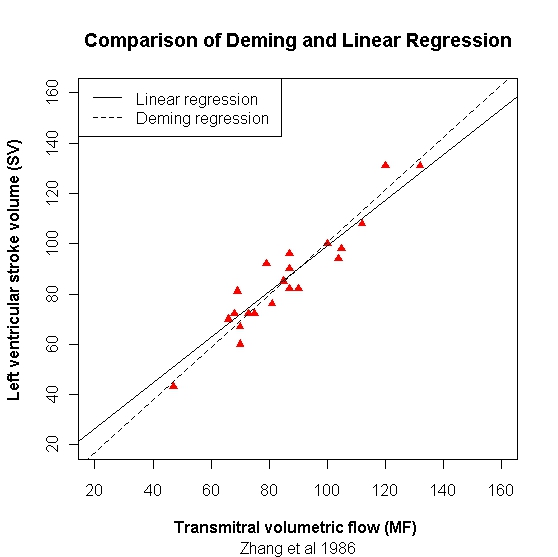
\includegraphics[width=130mm]{images/ZhangDeming.jpeg}
	\caption{Deming Regression For Zhang's Data}\label{ZhangDeming}
\end{figure}


\section{Model Evaluation for Deming Regression}
Bootstrap techniques can be used to obtain Confidence Intervals for Deming regression estimates. Authors such as 
\citet{carpenter2000bootstrap} and \citet{johnson2001bootstrap} provide relevant insights.




Model selection and diagnostic technique are well developed for classical linear regression methods. Typically an implementation of a linear model fit will be accompanied by additional information, such as the coefficient of determination and likelihood and information criterions, and a regression ANOVA table. Such additional information has not, as yet, been implemented for Deming regression.

Deming's Regression suffers from some crucial drawbacks. Firstly it is computationally complex, and it requires specific software packages to perform calculations. Secondly, in common with all regression methods, Deming regression is vulnerable to outliers. Lastly, Deming regression is uninformative
about the comparative precision of two methods of measurement. Most importantly \citet{CarollRupert} states that Deming's regression is acceptable only when the precision ratio ($\lambda$, in their paper as $\eta$) is correctly specified, but in practice this is often not the case, with the $\lambda$ being underestimated. This underestimation leads to an overcorrection for attenuation.


%===================================================%
\section{Other Proposals for Formal Testing}
\citet{Kinsella} notes the lack of formal testing offered by
this Bland-Altman plot. Furthermore, \citet{Kinsella} formulates a model for
single measurement observations as a
linear mixed effects model, i.e. a model that additively combines
fixed effects and random effects:
\[
Y_{ij} =\quad \mu + \beta_{j} + u_{i} + \epsilon_{ij} \qquad i = 1,\dots,n
\qquad j=1,2\]

The true value of the measurement is represented by $\mu$ while the fixed effect due to method $j$ is $\beta_{j}$.
For simplicity these terms can be combined into single terms; $\mu_{1} = \mu+ \beta_{1}$ and $\mu_{2} = \mu + \beta_{2}$. The inter-method bias is the difference of the two fixed effect terms, $\beta_{1}-\beta_{2}$. Each individual is assumed to give rise to a random error, represented by $u_{i}$. This random effects term is assumed to have mean zero and be normally distributed with variance $\sigma^2$. There is assumed to be an attendant error for each measurement on each individual, denoted $\epsilon_{ij}$. This is also assumed to have mean zero. The variance of measurement error for both methods are not assumed to be identical for both methods variance,  hence it is denoted $\sigma^2_{j}$. The set of observations ($x_{i},y_{i}$) by methods $X$ and $Y$ are assumed to follow a bivariate normal distribution with expected values $E(x_{i})= \mu_{i}$ and $E(y_{i})= \tau_{i}$ respectively. The variance covariance of the observations $\boldsymbol{\Sigma}$ is given by

\[
\boldsymbol{\Sigma} = \left[
\begin{array}{cc}
\sigma^{2} + \sigma^{2}_{1} & \sigma^{2} \\
\sigma^{2} & \sigma^{2} + \sigma^{2}_{2} \\
\end{array}
\right]
\] 
% The inter-method bias is the difference of the two fixed effect terms, $\beta_{1}-\beta_{2}$.

\citet{Kinsella} demonstrates the estimation of the variance terms and relative precisions relevant to a method comparison study, with attendant confidence intervals for both. The measurement model introduced by \citet{Grubbs48,Grubbs73} provides a formal procedure for estimating the variances $\sigma^2$, $\sigma^2_{1}$ and $\sigma^2_{2}$. \citet{Grubbs48} offers estimates, commonly known as Grubbs estimators, for the various variance components. These estimates are maximum likelihood estimates, which shall be revisited in due course.
\begin{eqnarray*}
	\hat{\sigma^{2}} = \sum{\frac{(x_{i}-\bar{x})(y_{i}-\bar{y})}{n-1}} = Sxy\\
	\hat{\sigma^{2}_{1}} = \sum{\frac{(x_{i}-\bar{x})^{2}}{n-1}} =S^{2}x - Sxy  \\
	\hat{\sigma^{2}_{2}} =
	\sum{\frac{(y_{i}-\bar{y})^{2}}{n-1}} = S^{2}y - Sxy
\end{eqnarray*}

% The standard error of these variance estimates are:
% \begin{eqnarray}
% \mbox{var}(\sigma^{2}_{1}) = \frac{2\sigma^{4}_{1}}{n-1} +
% \frac{\sigma^2_{S}\sigma^2_{1}+\sigma^2_{S}\sigma^2_{2}+\sigma^2_{1}\sigma^2_{2}
% }{n-1}\\
% \mbox{var}(\sigma^{2}_{2}) =\quad \frac{2\sigma^{4}_{2}}{n-1} +
% \frac{\sigma^2_{S}\sigma^2_{1}+\sigma^2_{S}\sigma^2_{2}+\sigma^2_{1}\sigma^2_{2}
% }{n-1}\nonumber
% \end{eqnarray}

\citet{Thompson} defines $\Delta_j = \sigma^2 / \sigma^2_j, j=1,2$, to be a measure of the
relative precision of the measurement methods, and demonstrates how to make statistical inferences about $\Delta_{j}$.
Based on the following identities,
\begin{eqnarray*}
	C_{x}&=&(n-1)S^2_{x},\nonumber\\
	C_{xy}&=&(n-1)S_{xy},\nonumber\\
	C_{y}&=&(n-1)S^2_{y},\nonumber\\
	|A| &=& C_{x}\times C_{y} - (C_{xy})^2,\nonumber
\end{eqnarray*}
\noindent the confidence interval limits of $\Delta_{1}$ are

\begin{eqnarray}
\frac{C_{xy}-
	t(\frac{|A|}{n-2})^{\frac{1}{2}}}{C_{x}-C_{xy}+
	t(\frac{|A|}{n-2})^{\frac{1}{2}}} <
\Delta_{1} < \frac{C_{xy}+
	t(\frac{|A|}{n-2})^{\frac{1}{2}}}{C_{x}-C_{xy}-
	t(\frac{|A|}{n-1})^{\frac{1}{2}}} \nonumber
\end{eqnarray}
The value $t$ is the $100(1-\alpha/2)\%$ upper quantile of
Student's $t$ distribution with $n-2$ degrees of freedom
\citep{Kinsella}. The confidence limits for $\Delta_{2}$ are found by substituting $C_{y}$ for $C_{x}$ in (1.2).
Negative lower limits are replaced by the value $0$.

%For the interval estimates for the variance components,
%\citet{Thompson} presents three relations that hold simultaneously
%with probability $1-2\alpha$ where $2\alpha=0.01$ or $0.05$.

%\begin{eqnarray*}
%|\sigma^2-C_{xy}K| &\leqslant& M(C_{x}C_{y})^{\frac{1}{2}}\\
%|\sigma^2_{1}-(C_{x}-C_{xy})K|&\leqslant M(C_{x}(C_{x}+C_{y}-2C_{xy}))^{\frac{1}{2}}\nonumber\\
%|\sigma^2_{2}-(C_{y}-C_{xy})K|&\leqslant
%M(C_{y}(C_{x}+C_{y}-2C_{xy}))^{\frac{1}{2}}\nonumber
%\end{eqnarray*}

%\citet{Thompson} contains tables for $K$ and $M$.

The case-wise differences and means are calculated as $d_{i} =
x_{i}-y_{i}$ and $a_{i} = (x_{i}+y_{i})/2$  respectively. Both
$d_{i}$ and $a_{i}$ are assumed to follow a bivariate normal
distribution with $E(d_{i})= \mu_{d} = \mu_{1} - \mu_{2}$ and
$E(a_{i})= \mu_{a} = (\mu_{1} + \mu_{2})/2$, and the variance matrix
$\Sigma_{(a,d)}$ is

\begin{eqnarray}
\Sigma_{(a,d)}= \left[\begin{matrix}
\sigma^{2}_{1}+\sigma^{2}_{2}&\frac{1}{2}(\sigma^{2}_{1}-\sigma^{2}_{2})\\
\frac{1}{2}(\sigma^{2}_{1}-\sigma^{2}_{2})&\sigma^{2}+
\frac{1}{4}(\sigma^{2}_{1}+\sigma^{2}_{2})
\end{matrix} \right].
\end{eqnarray}
\section{Formal Models and Tests}

\citet{Thompson} defines $\Delta_j = \sigma^2 / \sigma^2_j, j=1,2$, to be a measure of the
relative precision of the measurement methods, and demonstrates how to make statistical inferences about $\Delta_{j}$.
Based on the following identities,
\begin{eqnarray*}
	C_{x}&=&(n-1)S^2_{x},\nonumber\\
	C_{xy}&=&(n-1)S_{xy},\nonumber\\
	C_{y}&=&(n-1)S^2_{y},\nonumber\\
	|A| &=& C_{x}\times C_{y} - (C_{xy})^2,\nonumber
\end{eqnarray*}
\noindent the confidence interval limits of $\Delta_{1}$ are

\begin{eqnarray}
\frac{C_{xy}-
	t(\frac{|A|}{n-2}))^{\frac{1}{2}}}{C_{x}-C_{xy}+
	t(\frac{|A|}{n-2}))^{\frac{1}{2}}} <
\Delta_{1} < \frac{C_{xy}+
	t(\frac{|A|}{n-2}))^{\frac{1}{2}}}{C_{x}-C_{xy}-
	t(\frac{|A|}{n-1}))^{\frac{1}{2}}} \nonumber
\end{eqnarray}
The value $t$ is the $100(1-\alpha/2)\%$ upper quantile of
Student's $t$ distribution with $n-2$ degrees of freedom
\citep{Kinsella}. The confidence limits for $\Delta_{2}$ are found by substituting $C_{y}$ for $C_{x}$ in (1.2).
Negative lower limits are replaced by the value $0$.
The ratio $\Delta_{2}$
can be found by interchanging $C_{y}$ and $C_{x}$. A lower
confidence limit can be found by calculating the square root. The
inequality in equation $1.10$ may also be used for hypothesis
testing.


%For the interval estimates for the variance components,
%\citet{Thompson} presents three relations that hold simultaneously
%with probability $1-2\alpha$ where $2\alpha=0.01$ or $0.05$.

%\begin{eqnarray*}
%|\sigma^2-C_{xy}K| &\leqslant& M(C_{x}C_{y})^{\frac{1}{2}}\\
%|\sigma^2_{1}-(C_{x}-C_{xy})K|&\leqslant M(C_{x}(C_{x}+C_{y}-2C_{xy}))^{\frac{1}{2}}\nonumber\\
%|\sigma^2_{2}-(C_{y}-C_{xy})K|&\leqslant
%M(C_{y}(C_{x}+C_{y}-2C_{xy}))^{\frac{1}{2}}\nonumber
%\end{eqnarray*}

%\citet{Thompson} contains tables for $K$ and $M$.

%%%%%%%%%%%%%%%%%%%%%%%%%%%%%%%%%%%%%%%%%%%%%%%%%%%%%%%%%%%%%%%%%%%%%%%%%%%%%%%%%





%=================================================================%






\section{Thompson 1963: Model Formulation and Formal Testing}

\citet{Kinsella} formulates a model for un-replicated observations
for a method comparison study as a mixed model.
\begin{eqnarray}
Y_{ij} =\quad \mu_{j} + S_{i} + \epsilon_{ij} \quad i=1,2...n\quad
j=1,2\\
S \sim N(0,\sigma^{2}_{s})\qquad \epsilon_{ij} \sim
N(0,\sigma^{2}_{j}) \nonumber
\end{eqnarray}

As with all mixed models, the variance of each observation is the
sum of all the associated variance components.
\begin{eqnarray}
var(Y_{ij}) =\quad \sigma^{2}_{s} + \sigma^{2}_{j} \\
cov(Y_{i1},Y_{i2})=\quad \sigma^{2}_{s} \nonumber
\end{eqnarray}

As with all mixed models, the variance of each observation is the sum of all the associated variance components.
\begin{eqnarray}
var(Y_{ij}) =\quad \sigma^{2}_{s} + \sigma^{2}_{j} \\
cov(Y_{i1},Y_{i2})=\quad \sigma^{2}_{s} \nonumber
\end{eqnarray}

\citet{Grubbs48} offers maximum likelihood estimators, commonly
known as Grubbs estimators, for the various variance components:
\begin{eqnarray}
\hat{\sigma^{2}_{s}} \quad= \sum{\frac{(x_{i}-\bar{x})(y_{i}-\bar{y})}{n-1}}\quad=Sxy\\
\hat{\sigma^{2}_{1}} \quad= \sum{\frac{(x_{i}-\bar{x})^{2}}{n-1}} \quad=S^{2}x-Sxy \nonumber\\
\hat{\sigma^{2}_{2}} \quad=
\sum{\frac{(y_{i}-\bar{y})^{2}}{n-1}}\quad=S^{2}y-Sxy \nonumber
\nonumber
\end{eqnarray}

The standard error of these variance estimates are:
\begin{eqnarray}
var(\sigma^{2}_{1}) =\quad \frac{2\sigma^{4}_{1}}{n-1} +\quad
\frac{\sigma^2_{S}\sigma^2_{1}+\sigma^2_{S}\sigma^2_{2}+\sigma^2_{1}\sigma^2_{2}
}{n-1}\\
var(\sigma^{2}_{2}) =\quad \frac{2\sigma^{4}_{2}}{n-1} +\quad
\frac{\sigma^2_{S}\sigma^2_{1}+\sigma^2_{S}\sigma^2_{2}+\sigma^2_{1}\sigma^2_{2}
}{n-1}\nonumber
\end{eqnarray}


\citet{Kinsella} demonstrates the estimation of the variance terms and relative precisions relevant to a method comparison study, with attendant confidence intervals for both. The measurement model introduced by \citet{Grubbs48,Grubbs73} provides a formal procedure for estimating the variances $\sigma^2$, $\sigma^2_{1}$ and $\sigma^2_{2}$. \citet{Grubbs48} offers estimates, commonly known as Grubbs estimators, for the various variance components. These estimates are maximum likelihood estimates, which shall be revisited in due course.
\begin{eqnarray*}
	\hat{\sigma^{2}} = \sum{\frac{(x_{i}-\bar{x})(y_{i}-\bar{y})}{n-1}} = Sxy\\
	\hat{\sigma^{2}_{1}} = \sum{\frac{(x_{i}-\bar{x})^{2}}{n-1}} =S^{2}x - Sxy  \\
	\hat{\sigma^{2}_{2}} =
	\sum{\frac{(y_{i}-\bar{y})^{2}}{n-1}} = S^{2}y - Sxy
\end{eqnarray*}

% The standard error of these variance estimates are:
% \begin{eqnarray}
% \mbox{var}(\sigma^{2}_{1}) = \frac{2\sigma^{4}_{1}}{n-1} +
% \frac{\sigma^2_{S}\sigma^2_{1}+\sigma^2_{S}\sigma^2_{2}+\sigma^2_{1}\sigma^2_{2}
% }{n-1}\\
% \mbox{var}(\sigma^{2}_{2}) =\quad \frac{2\sigma^{4}_{2}}{n-1} +
% \frac{\sigma^2_{S}\sigma^2_{1}+\sigma^2_{S}\sigma^2_{2}+\sigma^2_{1}\sigma^2_{2}
% }{n-1}\nonumber
% \end{eqnarray}

The inter-method bias is the difference of the two fixed effect terms, $\beta_{1}-\beta_{2}$.

\citet{Kinsella} demonstrates how the Grubbs estimators for the
error variances can be calculated using the difference values,
providing a worked example on a data set.
\begin{eqnarray}
\hat{\sigma^{2}_{1}}
\quad=\sum{(y_{i1}-\bar{y{1}})(D_{i}-\bar{D})}\\
\hat{\sigma^{2}_{2}} \quad=
\sum{(y_{i2}-\bar{y_{2}})(D_{i}-\bar{D})} \nonumber
\end{eqnarray}

\citet{Thompson} presents confidence intervals for the relative
precisions of the measurement methods, $\Delta_{j}=
\sigma^2_{S}/\sigma^2_{j}$ (where $j=1,2$), as well as the
variances $\sigma^{2}_{S}, \sigma^{2}_{1}$ and $\sigma^{2}_{2}$.

\begin{eqnarray}
\Delta_{1} >\quad \frac{C_{xy}-
	t(|A|/n-2))^{\frac{1}{2}}}{C_{x}-C_{xy}+
	t(|A|/n-2))^{\frac{1}{2}}}
\end{eqnarray}
where

\begin{eqnarray}
C_{x}=\quad(n-1)S^2_{x}\nonumber\\
C_{xy}=\quad(n-1)S_{xy}\nonumber\\
C_{y}=\quad(n-1)S^2_{y}\nonumber\\
A=\quad C_{x}\times C_{y} - (C_{xy})^2 \nonumber
\end{eqnarray}

$t$ is the $100(1-\alpha/2)\%$ quantile of Student's $t$
distribution with $n-2$ degrees of freedom. $\Delta_{2}$ can be
found by changing $C_{y}$ for $C_{x}$. A lower confidence limit
can be found by calculating the square root. This inequality may
also be used for hypothesis testing.

\citet{Thompson} presents three relations that hold simultaneously
with probability $1-2\alpha$ where $2\alpha=0.01$ or $0.05$. \citet{Thompson} contains tables for $K$ and $M$.

\begin{eqnarray}
|\sigma^2-C_{xy}K|\leqslant M(C_{x}C_{y})^{\frac{1}{2}}\\
|\sigma^2_{1}-(C_{x}-C_{xy})K|\leqslant M(C_{x}(C_{x}+C_{y}-2C_{xy}))^{\frac{1}{2}}\nonumber\\
|\sigma^2_{2}-(C_{y}-C_{xy})K|\leqslant
M(C_{y}(C_{x}+C_{y}-2C_{xy}))^{\frac{1}{2}}\nonumber
\end{eqnarray}	








\section{Structural Equation Modelling}

Structural Equation modelling is a statistical technique used for testing and estimating causal relationships using a combination of statistical data and qualitative causal assumptions. \citet{carrasco2004} describes the structural equation model is a regression approach that allows to estimate a linear 
regression when independent variables are measured with error .
The structural equations approach avoids the biased estimation of the slope and intercept that occurs in ordinary least square regression.


 Several authors, such as \citet{Lewis}, \citet{gkelly1985},\citet{voelkel2005} and \citet{hopkins2004bias} advocate the use of SEM methods for method comparison. In \citet{hopkins2004bias}, a critique of the Bland-Altman plot he makes the following remark:

Authors, such as a \citet{lewis}, \citet{dunnSEME} and \citet{voelkel2005center}, strongly advocate the use of \textit{Structural Equation Models} for the purposes of method comparison. Conversely \citet{BA99} also states that consider structural equation models to be inappropriate.

\emph{What's needed for a comparison of two or more measures is a
	generic approach more powerful even than regression to model the
	relationship and error structure of each measure with a latent
	variable representing the true value.}

Hopkins also adds that he himself is collaborating in research utilising SEM and Mixed Effects modelling. \citet{gkelly1985} advised that \textit{the Structural equations model is used to estimate the linear relationship between new and standards method.
The Delta method is used to find the variance of the estimated parameters} \citep{gkelly1985}.


However Bland and Altman (1987) contends that it is unnecessary to perform elaborate statistical analysis, while also criticizing the SEM approach on the basis that it offers insights  on inter-method bias only, and not the variability about the line of equality. 
\begin{quote}
\textit{	However, it is quite wrong to argue solely from a lack of bias that two methods can be regarded as comparable...
Knowing the data are consistent with a structural equation with a slope of 1 says something 
about the absence of bias but nothing about the variability about Y = X (the difference between the measurements), which, as has already been stated, is all that really matters.}
\end{quote}
%-------------------------------------------------------------%





\chapter{Error In Variable Models}



\section{Background} 
In method comparison studies, it is of importance to assure that the presence of a difference of medical importance is detected. 
For a given difference, the necessary number of samples depends on the range of values and the analytical standard deviations of the methods involved. For typical examples, the present study evaluates the statistical power of least-squares and Deming regression analyses applied to the method comparison data.






\section{Model I and II Regression}

On account of the fact that one set of measurements are linearly related to another, one could surmise that Linear Regression is the most suitable approach to analyzing comparisons. This approach is unsuitable on two counts. Firstly one of the assumptions of Regression analysis is that the independent variable values are without error. 

In method comparison studies one must assume the opposite; that there is error present in the measurements. Secondly a regression of X on Y would yield and entirely different result from Y on X.

Model I regression is unsuitable for method comparison studies. Even in the case where one method is a gold standard , it is disputed as to whether it is a valid approach. 

Model II regression is suitable for method comparison studies, but it is more difficult to execute. Both Model I and II regression models are unduly influenced by outliers.



\citet{CornCoch} argue for the use of methods that based on
the assumption that both methods are imprecisely measured ,and
that yield a fitting that is consistent with both '$X$ on $Y$' and
'$Y$ on $X$' formulations. These methods uses alternatives to the
OLS approach to determine the slope and intercept.

They describe three such alternative methods of regression; Deming, Mandel, and Bartlett regression. Collectively the authors refer to these approaches as Model II regression techniques.

\begin{itemize}
	\item The authors make the distinction between model I and model II regression types.
	\item Model II regression is the appropriate type when the predictor variable “x” is measured with imprecision.
	Cornbleet and Cochrane remark that clinical laboratory measurements usually increase in absolute imprecision when larger values are measured. % - [**]
\end{itemize}

\begin{itemize}
	\item Model II regression is the appropriate type when the predictor variable “x” is measured with imprecision.
	Cornbleet and Cochrane remark that clinical laboratory measurements usually increase in absolute imprecision when larger values are measured. % - [**]
\end{itemize}
\subsection{Model I regression [Criterion v Test]}
\citet{CornCoch} define this analysis as the case in which the independent variable, X, is measured without error, with y as the dependent variable.
 
 

Simple Linear Regression is well known statistical technique, wherein estimates for slope and
intercept of the line of best fit are derived according to the Ordinary Least Square (OLS) principle. This method is known to \citet{CornCoch} as Model I regression.

Simple linear regression is defined as such with the name `Model I regression' by \citet{CornCoch}, in contrast to 'Model II regression'.

 
\subsection{Model II regression [Test V Test]}
In this type of analysis, both of the measurement methods are test methods, with both expected to be subject to error. Deming regression is an approach to model II regression.



In Model I regression, the independent variable is assumed to be
measured without error. For method comparison studies, both sets of measurement must be assumed to be measured with imprecision and neither case can be taken to be a reference method. Arbitrarily
selecting either method as the reference will yield two conflicting outcomes. A fitting based on '$X$ on $Y$' will give inconsistent results with a fitting based on '$Y$ on $X$'. Consequently model I regression is inappropriate for such cases.


    % 1.A. Use of SLR, description of SLR as Model I
    % 1.B. Inappropriate for MCS
    % 1.C  Calibration and Conversion problems

 
Simple linear regression calculates a line of best fit for two
sets of data, n which the independent variable, X, is measured without error, with y as the dependent variable.  

SLR (Model I) regression is considered by many \citet{BA83,CornCoch,ludbrook97} to be wholly unsuitable for
method comparison studies, although recommended for use in calibration studies [Corncoch]. Even in the case where one
method is a gold standard , it is disputed as to whether it is a valid approach. Model II regression is more suitable for method comparison studies, but it is more difficult to execute. Both Model I and II regression models are unduly influenced by outliers. Regression Models can not be used to analyze repeated measurements


Conversely, \citet{CornCoch} state that when the independent
variable $X$ is a precisely measured reference method, Model I
regression may be considered suitable. They qualify this statement
by referring the $X$ as \emph{the correct value}, tacitly
implying that there must still be some measurement error present.
The validity of this approach has been disputed elsewhere.

This regression method also calculates a line of best fit for two sets of data. It differs from Model I regression in that it is derived in a way that factors in for error in the x-axis, as well as the y-axis. \citet{CornCoch} refer to it as 'Model II regression'.

%\subsection{Cornbleet - Cochran }
Model II regression method also calculates a line of best fit for two sets of data. It differs from Model I regression in that it is derived in a way that factors in for error in the x-axis, as well as the y-axis. \citet{CornCoch} refer to it as 'Model II regression'.

\begin{itemize}
	\item Model II regression [Test V Test] In this type of analysis, both of the measurement methods are test methods, with both expected to be subject to error. Deming regression is an approach to model II regression.
	
	\item Model I regression [Criterion v Test] \citet{CornCoch} define this analysis as the case in which the independent variable, X, is measured without error, with $Y$ as the dependent
	variable.
	
	\item In method comparison studies, the X variable is a precisely measured reference method. In the \citet{CornCoch} paper It is argued that criterion may be regarded as the correct value.
	Other papers dispute this.
\end{itemize}


%%%%%%%%%%%%%%%%%%%%%%%%%%%%%%%%%%%%%%%%%%%%%%%%%%%%%%%%%%%%%%%%%%%%%%%%%
%6 Regression Based Approaches          %%%%%%%%%%%%%%%%%%%%%%%%%%%%%%%%%
\subsection{Contention }
Several papers have commented that this approach is undermined
when the basic assumptions underlying linear regression are not
met, the regression equation, and consequently the estimations of
bias are undermined. Outliers are a source of error in regression
estimates.


In method comparison studies, the X variable is a precisely measured reference method. In the \citet{CornCoch} paper. It is argued that criterion may be regarded as the correct value. Other papers dispute this.






\section{Deming Regression}
The appropriate estimates were derived by Kummel (1879), but were popularized in the context of medical statistics and clinical chemistry by Deming (1943).



% 1. SLR
% 2. EinV Regression
% 3. Deming Regression
% 4. Advanced Regression Methods



\section{Error-In-Variable Models for Regression}






%Significant error in the least-squares slope estimation occurs when the ratio of the standard deviation of measurement of a single x value to the standard deviation of the indepedent variable data set exceeds 0.2.

%Errors in the least-squares coefficients attributable to outliers can be avoided by eliminating data points whose vertical distance from the regression line exceed four times the standard error the estimate.





%======================================================= %

\subsection{Compuational Aspects of Deming Regression}









As stated previously, the fundamental flaw of simple linear regression is that it allows for measurement error in one variable only. This causes a downward biased slope estimate.



%-----------------------------------------------------------------------------------------------%


\subsection{Variance Ratio}

	


The Deming regression line is estimated by minimizing the sums of squared deviations in both the x and y directions at an angle determined by the ratio of the analytical standard deviations for the two methods.

In cases involving only single measurements by each method, $\lambda$ may be unknown and is therefore assumes a value of one. While this will bias the estimates, it is less biased than ordinary linear regression.

This ratio can be estimated if multiple measurements were taken with each method, but if only one measurement was taken with each method, it can be assumed to be equal to one.




%================================================================================================= %






\subsection{Estimating the Variance ratio}


\begin{eqnarray*}
	x_{i} = \mu +  \beta_{0} + \epsilon_{xi}\\
	y_{i} = \mu +  \beta_{1} + \epsilon_{yi}\\
\end{eqnarray*}
The inter-method bias is the difference of these biases. In order to determine an estimate for the residual variances, one of the method biases must be assumed to be zero, i.e. $\beta_{0} = 0$. The inter-method bias is now represented by $\beta_{1}$.

\begin{eqnarray*}
	x_{i} &=& \mu + \epsilon_{xi}\\
	y_{i} &=& \mu +  \beta_{1} + \epsilon_{yi}\\
\end{eqnarray*}

The residuals can be expressed as
\begin{eqnarray*}
	\epsilon_{xi} &=& x_{i} - \mu  \\
	\epsilon_{yi} &=& y_{i} - (\mu + \beta_{1}) \\
\end{eqnarray*}

The variance of the residuals are equivalent to the variance of the corresponding observations, $\sigma^{2}_{\epsilon x} =
\sigma^{2}_{x}$ and $\sigma^{2}_{\epsilon y} = \sigma^{2}_{y}$.
\begin{equation}
\lambda = \frac{\sigma^{2}_{yx}}{\sigma^{2}_{y}}.
\end{equation}

Assuming constant standard deviations, and given duplicate measurements, the analytical standard deviations are given by

\begin{eqnarray*}
	SD^{2}_{ax} = \frac{1}{2n} \sum (x_{2i} - x_{1i})^{2}\\
	SD^{2}_{ay} = \frac{1}{2n} \sum (y_{2i} - y_{1i})^{2}\\
\end{eqnarray*}

Using duplicate measurements, one can estimate the analytical
standard deviations and compute their ratio. This ratio is then
used for computing the slope by the Deming method.[Linnet]


%\section{performance in the presence of oultiers}
%All least square estimation methods are sensitive to outliers.

\subsection{Inferences for Deming Regression}
% - http://www.medcalc.org/manual/deming_regression.php
The Intercept and Slope are calculated according to Combleet \& Gochman, 1979. The standard errors and confidence intervals are estimated using the jackknife method (Armitage et al., 2002).

The 95\% confidence interval for the Intercept can be used to test the hypothesis that A=0. This hypothesis is accepted if the confidence interval for A contains the value 0. If the hypothesis is rejected, then it is concluded that A is significantly different from 0 and both methods differ at least by a constant amount.

The 95\% confidence interval for the Slope can be used to test the hypothesis that B=1. This hypothesis is accepted if the confidence interval for B contains the value 1. If the hypothesis is rejected, then it is concluded that B is significantly different from 1 and there is at least a proportional difference between the two methods.






\subsection{Expaning the use of Deming Regression for MCS}
As noted before, Deming regression is an important and informative methodology in method comparison studies.
For single measurement method comparisons, Deming regression offers a useful complement to LME models.












\section{Performance in the presence of outliers}
All least square estimation methods are sensitive to outliers.
In common with all regression methods, Deming regression is vulnerable to outliers. 

Bland Altman's 1986 paper contains a data set, measurement of mean velocity of circumferential fibre shortening (VCF) by the long axis and short axis in M-mode echocardiography. Evident in this data set are outliers. Choosing the most noticeable, we shall use the deming regression method on this data set, both with and
without this outlier, to assess its influence.
\begin{itemize}
	\item In the presence of the outlier, the intercept and slope are estimated to be $-0.0297027$ and $1.0172959$ respectively.
	\item Without the outlier the intercept and slope are estimated to be
	$-0.11482220$ and  $1.09263112$ respectively.
	\item We therefore conclude that Deming Regression is adversely affected
	by outliers , in the same way model I regression is.
\end{itemize}

%------------------------------------------------%









%\subsubsection*{Guidelines}
%Always plot the data. Suspected outliers may be identified from the scatter plot.
%$S_{ex}$  represents the precision of a single x measurement near the mean value of X
%\[\lambda = \frac{S^2_{ex}}{S^2_{ey}}\]
%%=========================================================================================================== %






\section{Using LME models to estimate the ratio (BXC) }

\begin{eqnarray*}
	y_{mi} &=& \mu + \beta_{m} + b_{i} + \epsilon_{mi}\\
\end{eqnarray*}

with $\beta_{m}$ is a fixed effect for the method $m$ and $b_{i}$ is a random effect associated with patient $i$, and
$\epsilon_{mi}$ as the measurement error. This is a simple single level LME model. \citet{pb} provides for the implementation of fitting a model. The variance ratio of the residual variances is immediately determinable from the output. This variance ratio can be use to fit a Deming regression, as described in chapter 1.






\section{Linnet - References}
The statistical procedures are described in:
Linnet K. Necessary sample size for method comparison studies based on regression analysis. Clin Chem 1999; 45: 882-94.
Linnet K. Performance of Deming regression analysis in case of misspecified analytical error ratio in method comparison studies. Clin Chem 1998; 44: 1024-1031.
Linnet K. Evaluation of regression procedures for methods comparison studies. Clin Chem 1993; 39. 424-432.
Linnet K. Estimation of the linear relationship between measurements of two methods with proportional errors. Stat Med 1990; 9: 1463-1473.



%============================================================================= %





\section{Ordinary Least Product Regression}
\citet{ludbrook97} states that the grouping structure can be
straightforward, but there are more complex data sets that have a hierarchical(nested) model.

Observations between groups are independent, but observations
within each groups are dependent because they belong to the same
subpopulation. Therefore there are two sources of variation:
between-group and within-group variance.
% \vspace{5 mm} \noindent Mean correction is a method of reducing
%bias.
%-------------------------------------------------




\section{Least Products Regression}
Used as an alternative to Bland-Altman Analysis, this method is also known as 'Geometric Mean Regression' and 'Reduced Major Axis Regression'. This regression model minimizes the areas of the right triangles formed by the data points' vertical and horizontal deviations from the fitted line and the fitted line.

 Model II regression analysis caters for cases in which random error is attached to both dependent and independent variables. Comparing methods of measurement is just such a case.(Ludbrook)
	
 Least products regression is the reviewer's preferred technique for analysing the Model II case. In this, the sum of the products of the vertical and horizontal deviations of the x,y values from the line is minimized.
	
 Least products regression analysis is suitable for calibrating one method against another. It is also a sensitive technique for detecting and distinguishing fixed and proportional bias between
	methods.

Least-products regression can lead to inflated SEEs and estimates that do not tend to their true values an N approaches infinity (Draper and Smith, 1998).



\bibliographystyle{chicago}
\bibliography{DB-txfrbib}
\end{document}
